\documentclass[12pt]{article}

\usepackage[margin=1in]{geometry}
\usepackage{amsfonts,amssymb,amsthm,amsmath,graphicx}
\usepackage{float}
\usepackage{listings}
\usepackage{hyperref}
\usepackage{verbatim}
\usepackage{mathtools}
\usepackage{enumitem}
\usepackage{xcolor}
\usepackage{algorithm, algpseudocode, algorithmicx}

% Line Comment environment for algorithm environments.
\algnewcommand{\LineComment}[1]{\State \(\triangleright\) #1}

\hypersetup{
    colorlinks,
    linkcolor={red!50!black},
    citecolor={blue!50!black},
    urlcolor={blue!80!black}
}

\definecolor{boxbackground}{rgb}{1,0.976, 0.882}

\lstset{
    language=Python,
    basicstyle=\scriptsize\ttfamily,
    keywordstyle=\color{blue}\ttfamily,
    stringstyle=\color{red}\ttfamily,
    commentstyle=\color{green!50!black}\ttfamily,
    frame=single,
    breaklines=true,
    postbreak=\raisebox{0ex}[0ex][0ex]{\ensuremath{\color{violet}\hookrightarrow\space}},
    backgroundcolor = \color{boxbackground},
    showspaces=false,
    showstringspaces=false,
}

\newcommand{\N}{\mathbb{N}}
\newcommand{\Z}{\mathbb{Z}}
\newcommand{\R}{\mathbb{R}}
\newcommand{\Q}{\mathbb{Q}}
\newcommand{\e}{\epsilon}
\newcommand{\C}{\mathbb{C}}
\newcommand{\norm}[1]{\left\lVert#1\right\rVert}
\newcommand{\li}[1]{\lstinline[prebreak=]!#1!}
\newcommand{\p}[1]{\left(#1\right)}
\DeclareMathOperator*{\argmax}{\arg\,max}

\begin{document}
\title{Naive Bayes Classification}
\author{Amelia Henriksen}
\maketitle

\begin{comment}
\section*{What is Naive Bayes?}
\subsection*{Multinomial Naive Bayes}
\subsection*{Gaussian Naive Bayes}

\section*{Possible Improvements to the Algorithm}

\section*{Results}
\subsection*{The Seeds Dataset}
% Include pretty pictures of the initial awesomeness here

\subsection*{Comparison to the industrial implementation}
\end{comment}

A Naive Bayes classifier is a simple and accessible model that has numerous applications: from text classification to medical diagnostics. 
Naive Bayes has essentially two parts: application of Bayes theorem and a strong independence assumption.
To describe the algorithm and how it works, we will discuss it in the context of a very simple classification problem.
\section*{The Problem}
Suppose we want to build a classifier based on the ``seeds'' dataset found in the UCI Machine Learning repository \cite{Lichman}.
This dataset consists of 210 randomly selected samples of wheat kernels with seven measurements for associated geometric features.
These real valued, continuous features indicate the area, perimeter, compactness, length, width, asymmetry coefficient, and length of the kernel groove for each kernel sample.
Furthermore, each kernel is classified by one of three varieties of wheat: Kama, Rosa, or Canadian. 
We call these three classifications our ``label set.''

Given a single wheat kernel's feature measurements, we want to predict its associated label.
Let $x = (x_1, x_2, \ldots x_n)$ be a sample with $n$ features (note that for the seeds dataset, $n = 7$). 
Let $Y = \{y_1, \ldots, y_m\}$ be the label set (for the seeds dataset, $m=3$).
For each label $y_j$ in the label set, we want to compute the probability of the sample $x$ having a given label.
Naive Bayes finds the label $y_j$ that maximizes $P(y_j | x_1, x_2, \ldots, x_n)$ for all $y_j \in Y$ \cite{NaiveBayes}.

 We use Bayes' theorem to compute $$P(y_j|x_1, x_2 \ldots x_n) = \frac{P(x_1, x_2, \ldots, x_n|y_j) P(y_j)}{P(x_1, x_2, \ldots, x_n)}$$.
 Here is where the independence assumption comes into play. 
 We assume that the random variables associated with each feature $i$ are independent for all $i \in {1, \ldots, n}$.
This allows us to compute $$P(y_j|x_1, x_2, \ldots x_n) = \frac{P(y_j) \prod_{i=1}^n P(x_i|y_j)}{P(x_1, x_2, \ldots, x_n)}$$

Finally, we can compute the predicted label for our sample:
$$y = \argmax_{y_j \in Y} \frac{P(y_j) \prod_{i=1}^n P(x_i|y_j)}{P(x_1, x_2, \ldots, x_n)} = \argmax_{y_j \in \text{label set}}P(y_j) \prod_{i=1}^n P(x_i|y_j) $$
We avoid underflow by equivalently solving
$$y = \argmax_{y_j \in K}\log(P(y_j)) + \sum_{i=1}^n \log(P(x_i|y_j))$$

The assumption that the features of our dataset are independent of one another may seem rather strong--it is the reason Naive Bayes is considered ``naive.''
 Indeed, when we take a look at the features in the wheat dataset, we see a clear dependence between the area parameter and the length and width parameters. 
 However, as we will later see, the Naive Bayes classifier consistently yields surprisingly good results, even when the independence condition is violated.
 This, in conjunction with the relative simplicity of the algorithm, is what makes the method so powerful. 
 
\subsection*{Solving for $P(y_j)$ and $P(x_i|y_j)$}
We solve for $P(y_j)$ and $P(x_i|y_j)$ using a training dataset $X$, that is, using a set of samples with known labels.
We calculate $P(y_j)$ to be the probability that a sample of label $y_j$ appears in the training set. 
For example, in our seeds dataset, there are $70$ samples of Kama wheat kernels. 
Thus $P(Kama) = \frac{70}{210} = \frac{1}{3}$.


Since each feature in the seeds dataset is continuous and real valued, we decide to use the Gaussian distribution to model $P(x_i| y_j)$ for each $i \in \{1, \ldots, n\}, j \in \{1, \ldots, m\}$.
Note that although we will be demonstrating the efficacy of the Gaussian Naive Bayes classifier in this example, Multivariate and Bernouilli Naive Bayes classifiers are equally popular (indeed, Multinomial Naive Bayes is highly effective in text classification).
%%%%%%%%%%%%%% PUT A CITATION HERE %%%%%%%%%%%
We calculate each $P(x_i | y_j)$ by using the maximum likelihood estimator to determine the appropriate parameters for each label.
Thus, if there are $l$ samples in the training set with label $y_j$, and $\{X_{ki}\}_{k=1}^l$ is the set of measurements for feature $i$ on this set of samples, then $$\mu_{ji} = \frac{1}{l} \sum_{k=1}^l X_{ki}$$ and $$\sigma^2_{ji} = \frac{1}{l} \sum_{k=1}^l (X_{ki} - \mu_{ji})^2$$.
%Then, if $x_i$ is the measurement of our new sample for feature $i$, we can compute $$P(x_i | y_j) = f(x_i | \mu_{ij}, \sigma_{ij}^2) = \frac{1}{\sqrt
We can carry out similar MLE computations to find the estimated parameters for other distributions. 

Then, if $x_i$ is the sample measurement for feature $i$, we can compute  $$P(x_i | y_j) = f(x_i | \mu_{ji}, \sigma^2_{ji}) = \frac{1}{\sqrt{2 \sigma_{ji}^2 \pi}} e^{-\frac{(x_i - \mu_{ji})^2}{2 \sigma_{ji}^2}}$$

Finally, we predict the label for our sample $x$: 
\begin{align*}
y &= \argmax_{y_j \in Y}\log(P(y_j)) + \sum_{i=1}^n \log(P(x_i|y_j))\\
&= \argmax_{y_j \in Y}\log(P(y_j)) + \sum_{i=1}^n \log\p{\frac{1}{\sqrt{2 \sigma_{ji}^2 \pi}} e^{-\frac{(x_i - \mu_{ji})^2}{2 \sigma_{ji}^2}}}\\
&= \argmax_{y_j \in Y}\log(P(y_j)) + \sum_{i=1}^n \log\p{\frac{1}{\sqrt{2 \sigma_{ji}^2 \pi}}} + \log \p{ e^{-\frac{(x_i - \mu_{ji})^2}{2 \sigma_{ji}^2}}}\\
&= \argmax_{y_j \in Y}\log(P(y_j)) + \sum_{i=1}^n \log\p{\frac{1}{\sqrt{2 \sigma_{ji}^2 \pi}}} +  \p{-\frac{(x_i - \mu_{ji})^2}{2 \sigma_{ji}^2}}\\
\end{align*}

This generates the following algorithm for predicting the label of a sample $x$ using a Gaussian Naive Bayes classifier built with training data $X$ (where $X$ is a training set of $l$ samples with $n$ features with a known label for each sample)
The Multinomial and Bernoulli Naive Bayes algorithms follow similarly.

\subsubsection*{Gaussian Naive Bayes}
\begin{itemize}
    \item Fitting the training data:
    \begin{enumerate}
        \item Group the training data $X$ by label.
        \item For each label $y_j \in Y$
            \begin{enumerate}
                \item set $P(y_j) = \frac{\text{number of samples with label $y_j$}}{l}$
                \item For each feature $i \in \{1, \ldots, n\}$, calculate the MLE for the distribution parameters.
                \begin{align}
                \mu_{ji} &= \frac{1}{l} \sum_{k=1}^l X_{ki},\\ 
                \sigma^2_{ji} &= \frac{1}{l} \sum_{k=1}^l (X_{ki} - \mu_{ji})^2
                \end{align}
            \end{enumerate}
    \end{enumerate}
    \item Predicting the label for a sample $x = (x_1, \ldots, x_n)$
    \begin{enumerate}
        \item For each label $y_j \in Y$, calculate $\log(P(y_j)) + \sum_{i=1}^n \log{P(x_i | y_j)}$. 
        
         Calculate: $$ \log(P(y_j)) + \sum_{i=1}^n \log\p{\frac{1}{\sqrt{2 \sigma_{ji}^2 \pi}}} +  \p{-\frac{(x_i - \mu_{ji})^2}{2 \sigma_{ji}^2}}$$
        \item Return the label that maximizes the above sum
    \end{enumerate}
\end{itemize}

As we can see here, building a Naive Bayes classifier consists of three simple and straightforward pieces:
\begin{enumerate}
    \item Initializing a classifier object for a given label set
    \item Fitting the classifier to a training dataset with samples and labels
    \item Predicting the labels for a test set of samples.
\end{enumerate}

These pieces are what we use to computationally build up our Gaussian Naive bayes class, found in ``NaiveBayes.py''. 
The array functionality available in NumPy is particularly well suited to this problem, as NumPy's efficient array broadcasting allows us to compute the distribution parameters and prediction probabilities using cohesive array manipulations rather than costly for loops. 
Fancy indexing  and boolean masks also make returning and manipulating the labels for training data more effective and efficient.
Details are included in the documentation for ``NaiveBayes.py''

\section*{Results for GaussNaiveBayes class}
We now want to test our GaussNaiveBayes class for the ``seeds'' problem. 
These tests can be found in ``NaiveBayesTest.ipynb.''
We test the accuracy of our classifier by splitting the seeds dataset into a training set and a testing set for various test sizes and comparing the predicted test labels to the actual test labels (see self.accuracy in ``NaiveBayes.py''). 

To get a sense for the average accuracy of our predictions, we test 100 trials for each testsize, and in turn test 100 equally incremented testsizes between $0.01$ and $0.98$ ($1\%$ of the data to $98\%$ of the data).
To test the accuracy of our classifier against its industrial counterpart, we run the same procedure using the sklearn.naive\_bayes.GaussianNB object.
The results are shown in Figure 1, below.
\begin{figure}[H] 
    \centering
    \begin{minipage}[b]{0.6\textwidth}
    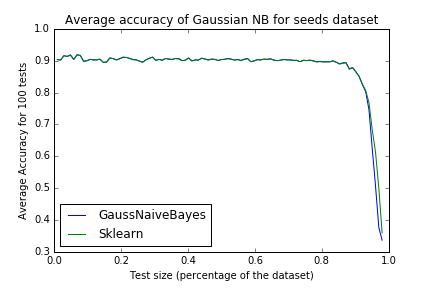
\includegraphics[width=\textwidth]{AvAccSeeds.png}
    \end{minipage}
    \caption{Accuracy of Gaussian Naive Bayes for the seeds dataset, for various test sizes. }
\end{figure}
This figure demonstrates some interesting results. 
First, recall that many of the features in our seeds dataset violated the independence assumption from which our classifier was derived.
Yet our GaussNaiveBayes class yields about 90$\%$ accuracy--a respectable score.
Even more impressive is the consistency of this accuracy--our model attains about $90\%$ average accuracy for classifiers trained on less than 20\% of the dataset (before dropping as the training dataset becomes insufficiently small, as we would expect to see).

We also note that our personal implementation for Naive Bayes matches the accuracy of the sklearn implementation exactly up to about .9 testsize, and closely in the test sizes following.
This testifies to the simplicity and efficacy of the test size.

In figure two, we take a closer look at the individual accuracies for each test run. 
As we can see here, the accuracy for the classifier has higher variation for trials of extremely small test sets--this could be explained by over-fitting ofthe model. 
Similarly, we see that the accuracy for the classifier has higher variation for trials of extremely large test sets--this could be explained by under-fitting of the model. 
Note that these accuracy scatter-plots match almost exactly between the industrial and personal Naive Bayes objects, with the industrial counterpart compensating slightly better for very small training datasets.

\begin{figure}[H] 
    \centering
    \begin{minipage}[b]{0.48\textwidth}
    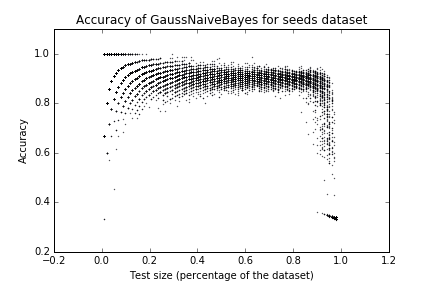
\includegraphics[width=\textwidth]{AccSeeds.png}
    \end{minipage}
    \quad
    \begin{minipage}[b]{0.48\textwidth}
    \includegraphics[width=\textwidth]{sklAccSeeds.png}
    \end{minipage}
    \caption{Accuracy of Gaussian Naive Bayes for the seeds dataset, for various test sizes. }
    %\label{fig:intro2}
\end{figure}
 
 Finally, we want to compare the timing between the industrial implementation of gaussian naive bayes and our personal class. 
 Using the magic $\%\% timeit$ function in the ipython notebook, we find that the GaussNaiveBayes class predict method is actually faster than it's sklearn counterpart (between 1/3 - 2/3 the time).
 For example, for a test size of $0.2$, we have the following results:
\begin{lstlisting}
 train, test = train_test_split(np.arange(y.size),test_size=.2)
Xtr, Xt, ytr, yt = X[train], X[test], y[train], y[test]
NB.fit(Xtr,ytr)
sklNB.fit(Xtr, ytr)
%%timeit
NB.fit(Xtr,ytr)
#>>> 10000 loops, best of 3: 192 micro s per loop

%%timeit
sklNB.fit(Xtr,ytr)
#>>>1000 loops, best of 3: 381 micro s per loop

%%timeit
p1 = NB.predict(Xt)
#>>>10000 loops, best of 3: 41.8 micro s per loop

%%timeit
p2 = sklNB.predict(Xt)
#>>>10000 loops, best of 3: 112 micro s per loop
 \end{lstlisting}
 Though this is likely due to some preprossessing and assertions on the part of the more robust sklearn function, which become important at higher dimensions, this still speaks highly to the efficiency of our implementation. 
 
 \section*{Improving Naive Bayes}


\bibliography{fp_references}
\bibliographystyle{unsrt}


\end{document} 